\subsection{Compute the crime rate per household. Generate a table of descriptive statistics of all the
variables that have been introduced so far. Comment on the descriptive statistics.}
% latex table generated in R 4.2.1 by xtable 1.8-4 package
% Wed Dec  6 21:45:13 2023
\begin{table}[ht]
\centering
\begin{tabular}{llllllr}
  \hline
var & median & mean & min & max & sd & NAs \\ 
  \hline
agro\_emp & 18.6 & 25.1 & 0.1 & 86.3 & 22.3 &  30 \\ 
  bribery & 11.7 & 17.0 & 0.0 & 67.1 & 14.7 &  87 \\ 
  gfce & 16.5 & 17.7 & 5.1 & 62.9 & 8.4 &  36 \\ 
  literacy & 93.0 & 83.6 & 24.2 & 100.0 & 19.3 &  61 \\ 
  log\_gdp & 9.4 & 9.3 & 6.6 & 11.6 & 1.2 &  22 \\ 
  pop\_total & 6.2e+06 & 3.4e+07 & 1.1e+04 & 1.4e+09 & 1.4e+08 &   2 \\ 
  self\_emp & 35.0 & 40.9 & 0.4 & 94.8 & 27.0 &  30 \\ 
  stocks & 6.4 & 28.8 & 0.0 & 538.7 & 66.8 & 131 \\ 
  sample\_size & 715.1 & 3.6e+03 & 120.1 & 1.4e+05 & 1.3e+04 &   2 \\ 
   \hline
\end{tabular}
\caption{Descriptive statistics} 
\label{desc}
\end{table}


Table \ref{desc2} shows the descriptive statistics of the table made of
900 hundred municipalities. First, the data is remarkably clean as their is no
NA values in it. For a clearer view I displayed the relative standard deviation (rsd)
defined as the standard deviation divided by the mean.
\subsection{Estimate the model in equation (7) using OLS.}

% Table created by stargazer v.5.2.3 by Marek Hlavac, Social Policy Institute. E-mail: marek.hlavac at gmail.com
% Date and time: Ven, déc 08, 2023 - 16:57:32
% Requires LaTeX packages: dcolumn 
\begin{table}[!htbp] \centering 
  \caption{Ordinary Least Square Estimation - Exercise 3} 
  \label{results2} 
\begin{tabular}{@{\extracolsep{5pt}}lD{.}{.}{-3} } 
\\[-1.8ex]\hline 
\hline \\[-1.8ex] 
 & \multicolumn{1}{c}{\textit{Dependent variable:}} \\ 
\cline{2-2} 
\\[-1.8ex] & \multicolumn{1}{c}{crime\_rate} \\ 
\hline \\[-1.8ex] 
 business\_crea & 0.018^{***} \\ 
  & (0.005) \\ 
  & \\ 
 log(pop) & 0.001^{***} \\ 
  & (0.0002) \\ 
  & \\ 
 income & 0.00001 \\ 
  & (0.0001) \\ 
  & \\ 
 com\_typeC & -0.003^{***} \\ 
  & (0.0003) \\ 
  & \\ 
 com\_typeI & -0.002^{***} \\ 
  & (0.001) \\ 
  & \\ 
 Constant & 0.001 \\ 
  & (0.002) \\ 
  & \\ 
\hline \\[-1.8ex] 
Observations & \multicolumn{1}{c}{899} \\ 
R$^{2}$ & \multicolumn{1}{c}{0.150} \\ 
Adjusted R$^{2}$ & \multicolumn{1}{c}{0.145} \\ 
Residual Std. Error & \multicolumn{1}{c}{0.004 (df = 893)} \\ 
F Statistic & \multicolumn{1}{c}{31.568$^{***}$ (df = 5; 893)} \\ 
\hline 
\hline \\[-1.8ex] 
\textit{Note:}  & \multicolumn{1}{r}{$^{*}$p$<$0.1; $^{**}$p$<$0.05; $^{***}$p$<$0.01} \\ 
\end{tabular} 
\end{table} 

The coefficient of interest that results from the OLS (see Table \ref{results2}) is significantly different from zero at the 1\% level, and positive.
This is very unexpected as it would mean that the better the shape of the economy, the higher the crime rate. This result
could derive from endogeneity issues as an ommited variable bias for instance.
The fact that the coefficient of interest is positive while we expect it to be negative
means that the endogeneity issues are more than just measurment error as this kind of
problem leads underestimations (in absolute value) of the true coefficient.

\subsection{After estimating the model in equation (7), you wonder whether enodegeneity is a problem.
Why could the variable of interest, the business creation growth rate, be endogenous?}
As mentioned in the previous question, the fact that the estimation for the coefficient of interest is positive
leads to thinking about an ommited variable bias. For instance, both the shape of the economy and the crime rate could
be related to the level of inequality in the area. To inspect this hypothesis, we used the
iqr\_income variable which is defined as the difference between the first and third quartiles of income.
This is a proxy for the local level of inequality. Figure \ref{ineq} displays the crime rate and the business creation growth rate
against the iqr\_income variable. Even though the result is not cristal clear, we still find some positive correlation for both
the dependant and the explanatory variable. This is a source of enodegeneity. The coefficient of correlation with iqr\_income are respectively 0.23 and 0.082 for the business creation rate and the crime rate. 
\begin{figure}[htbp]
    \begin{minipage}{0.5\textwidth}
      \centering
      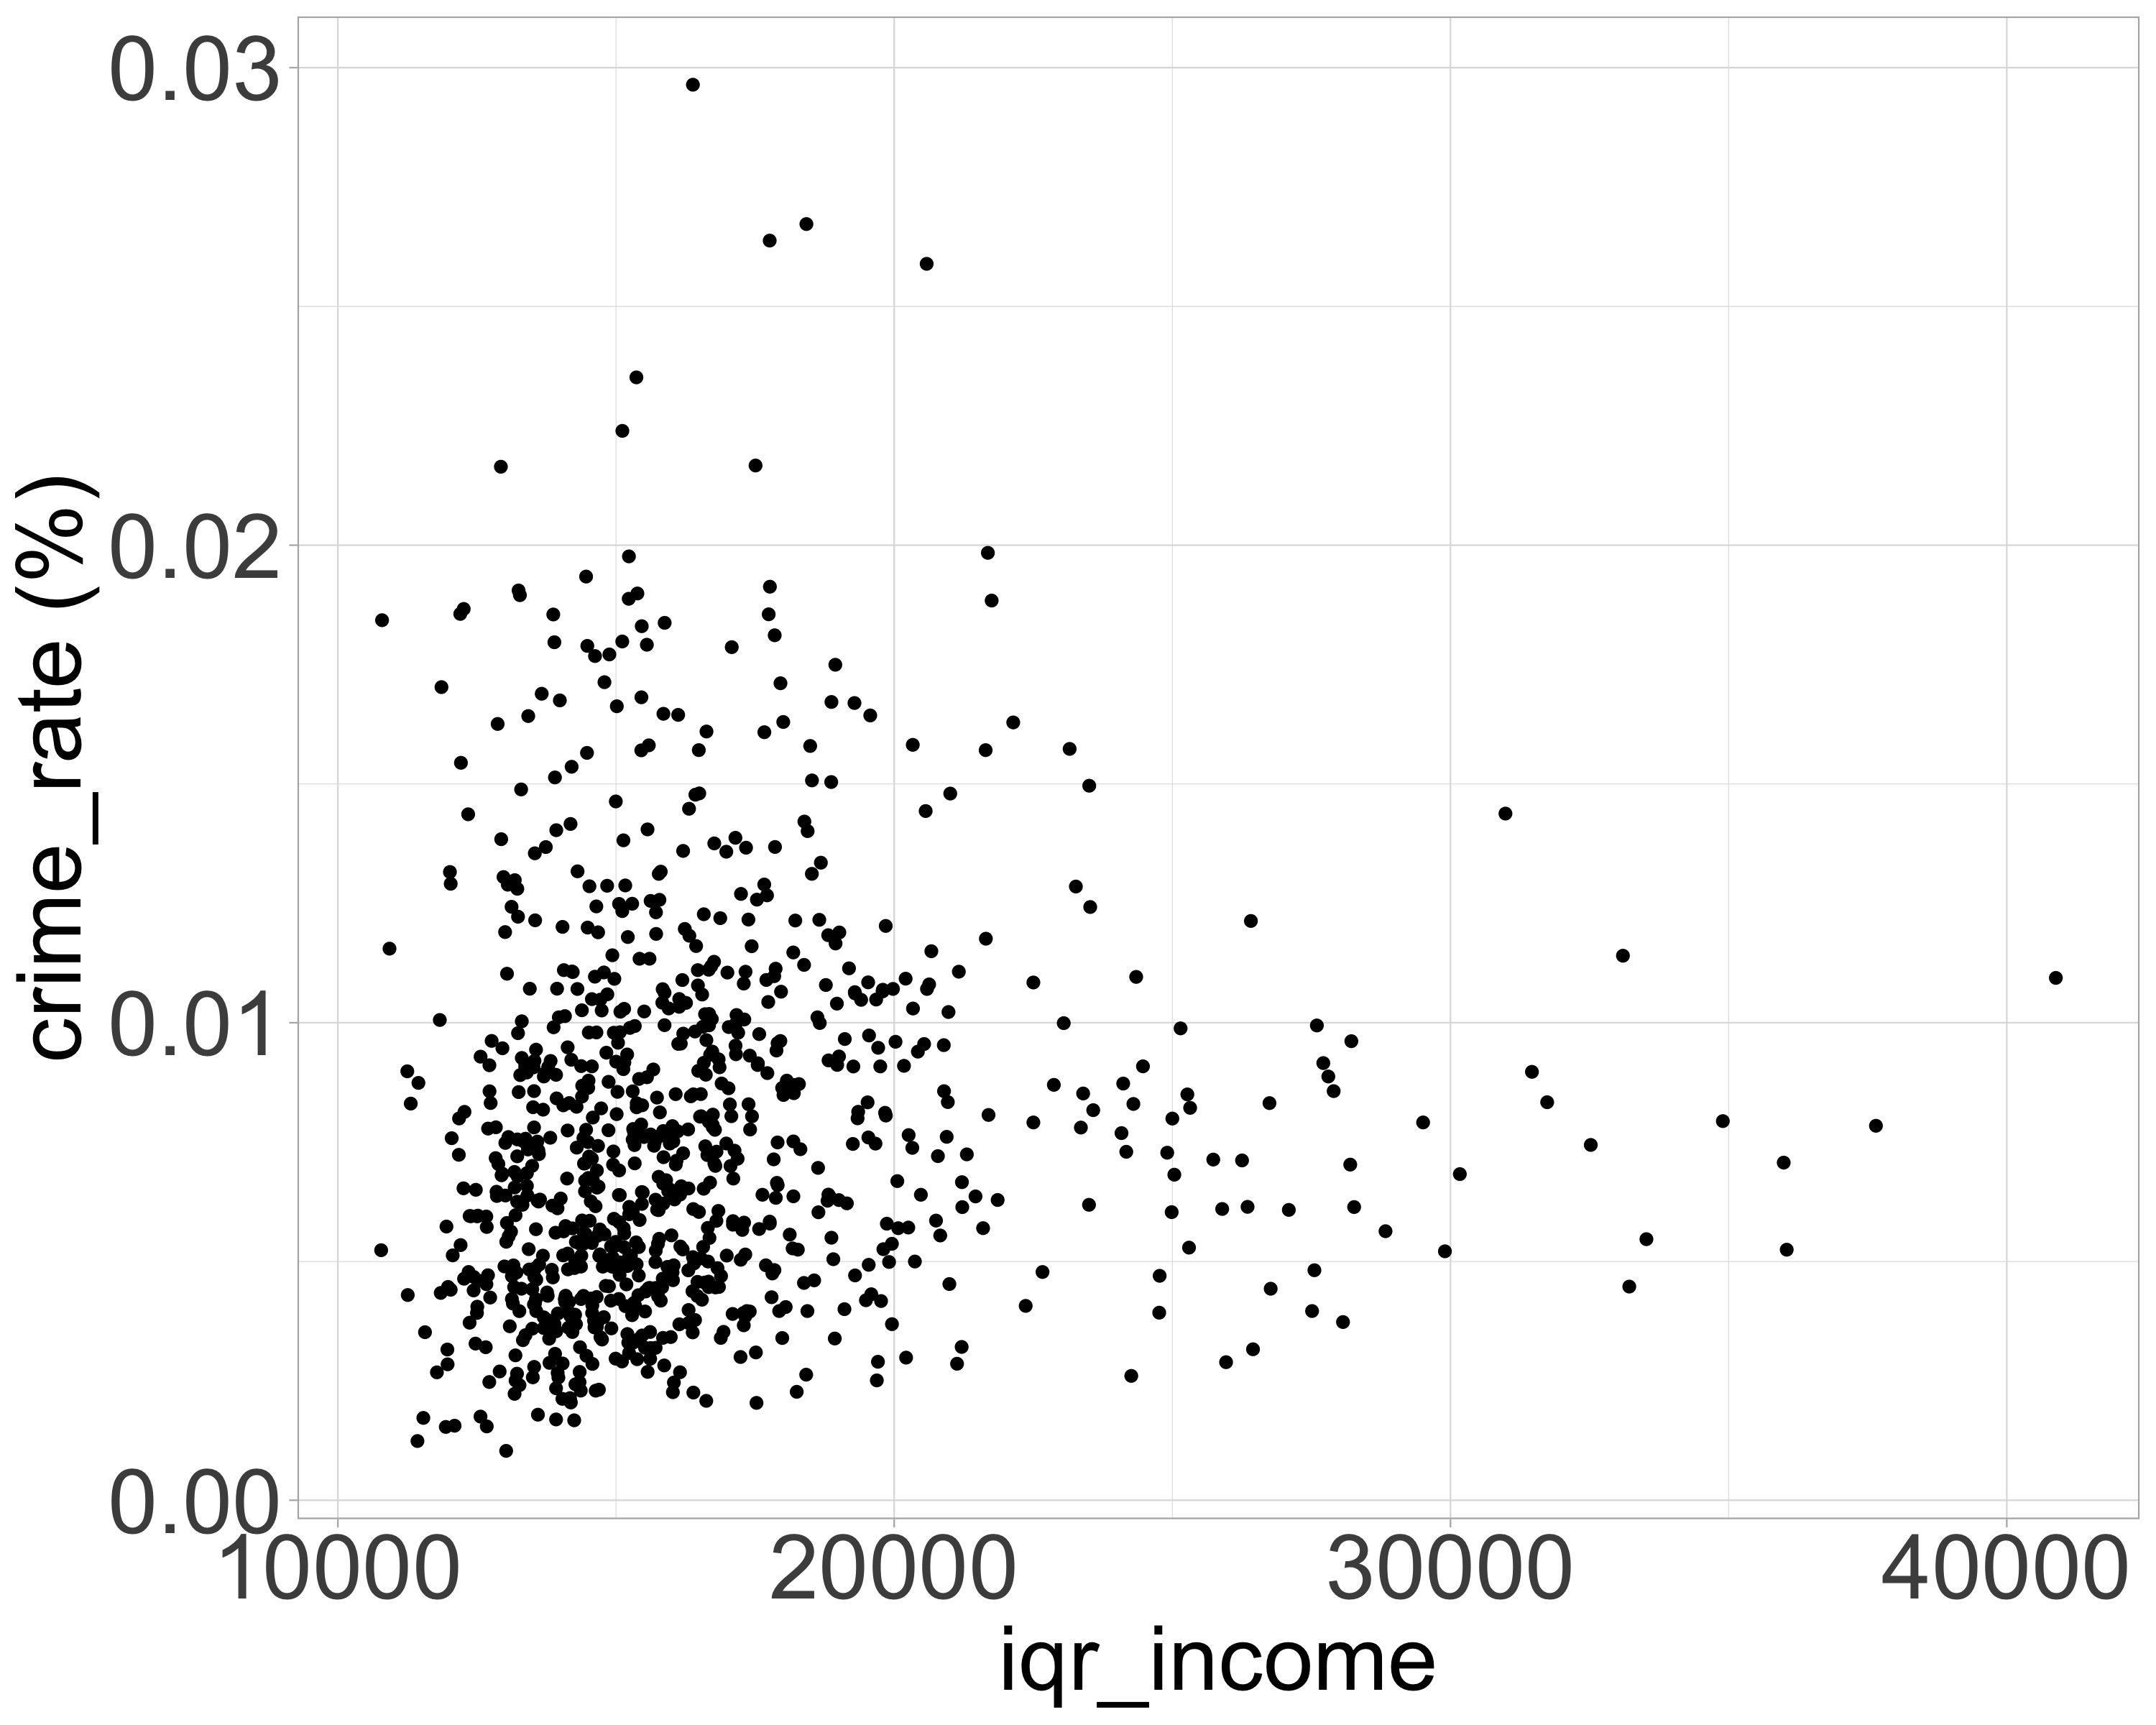
\includegraphics[width=\textwidth]{Exercise_3/OUTPUT/cr_iqr.png}
    \end{minipage}%
    \begin{minipage}{0.5\textwidth}
      \centering
      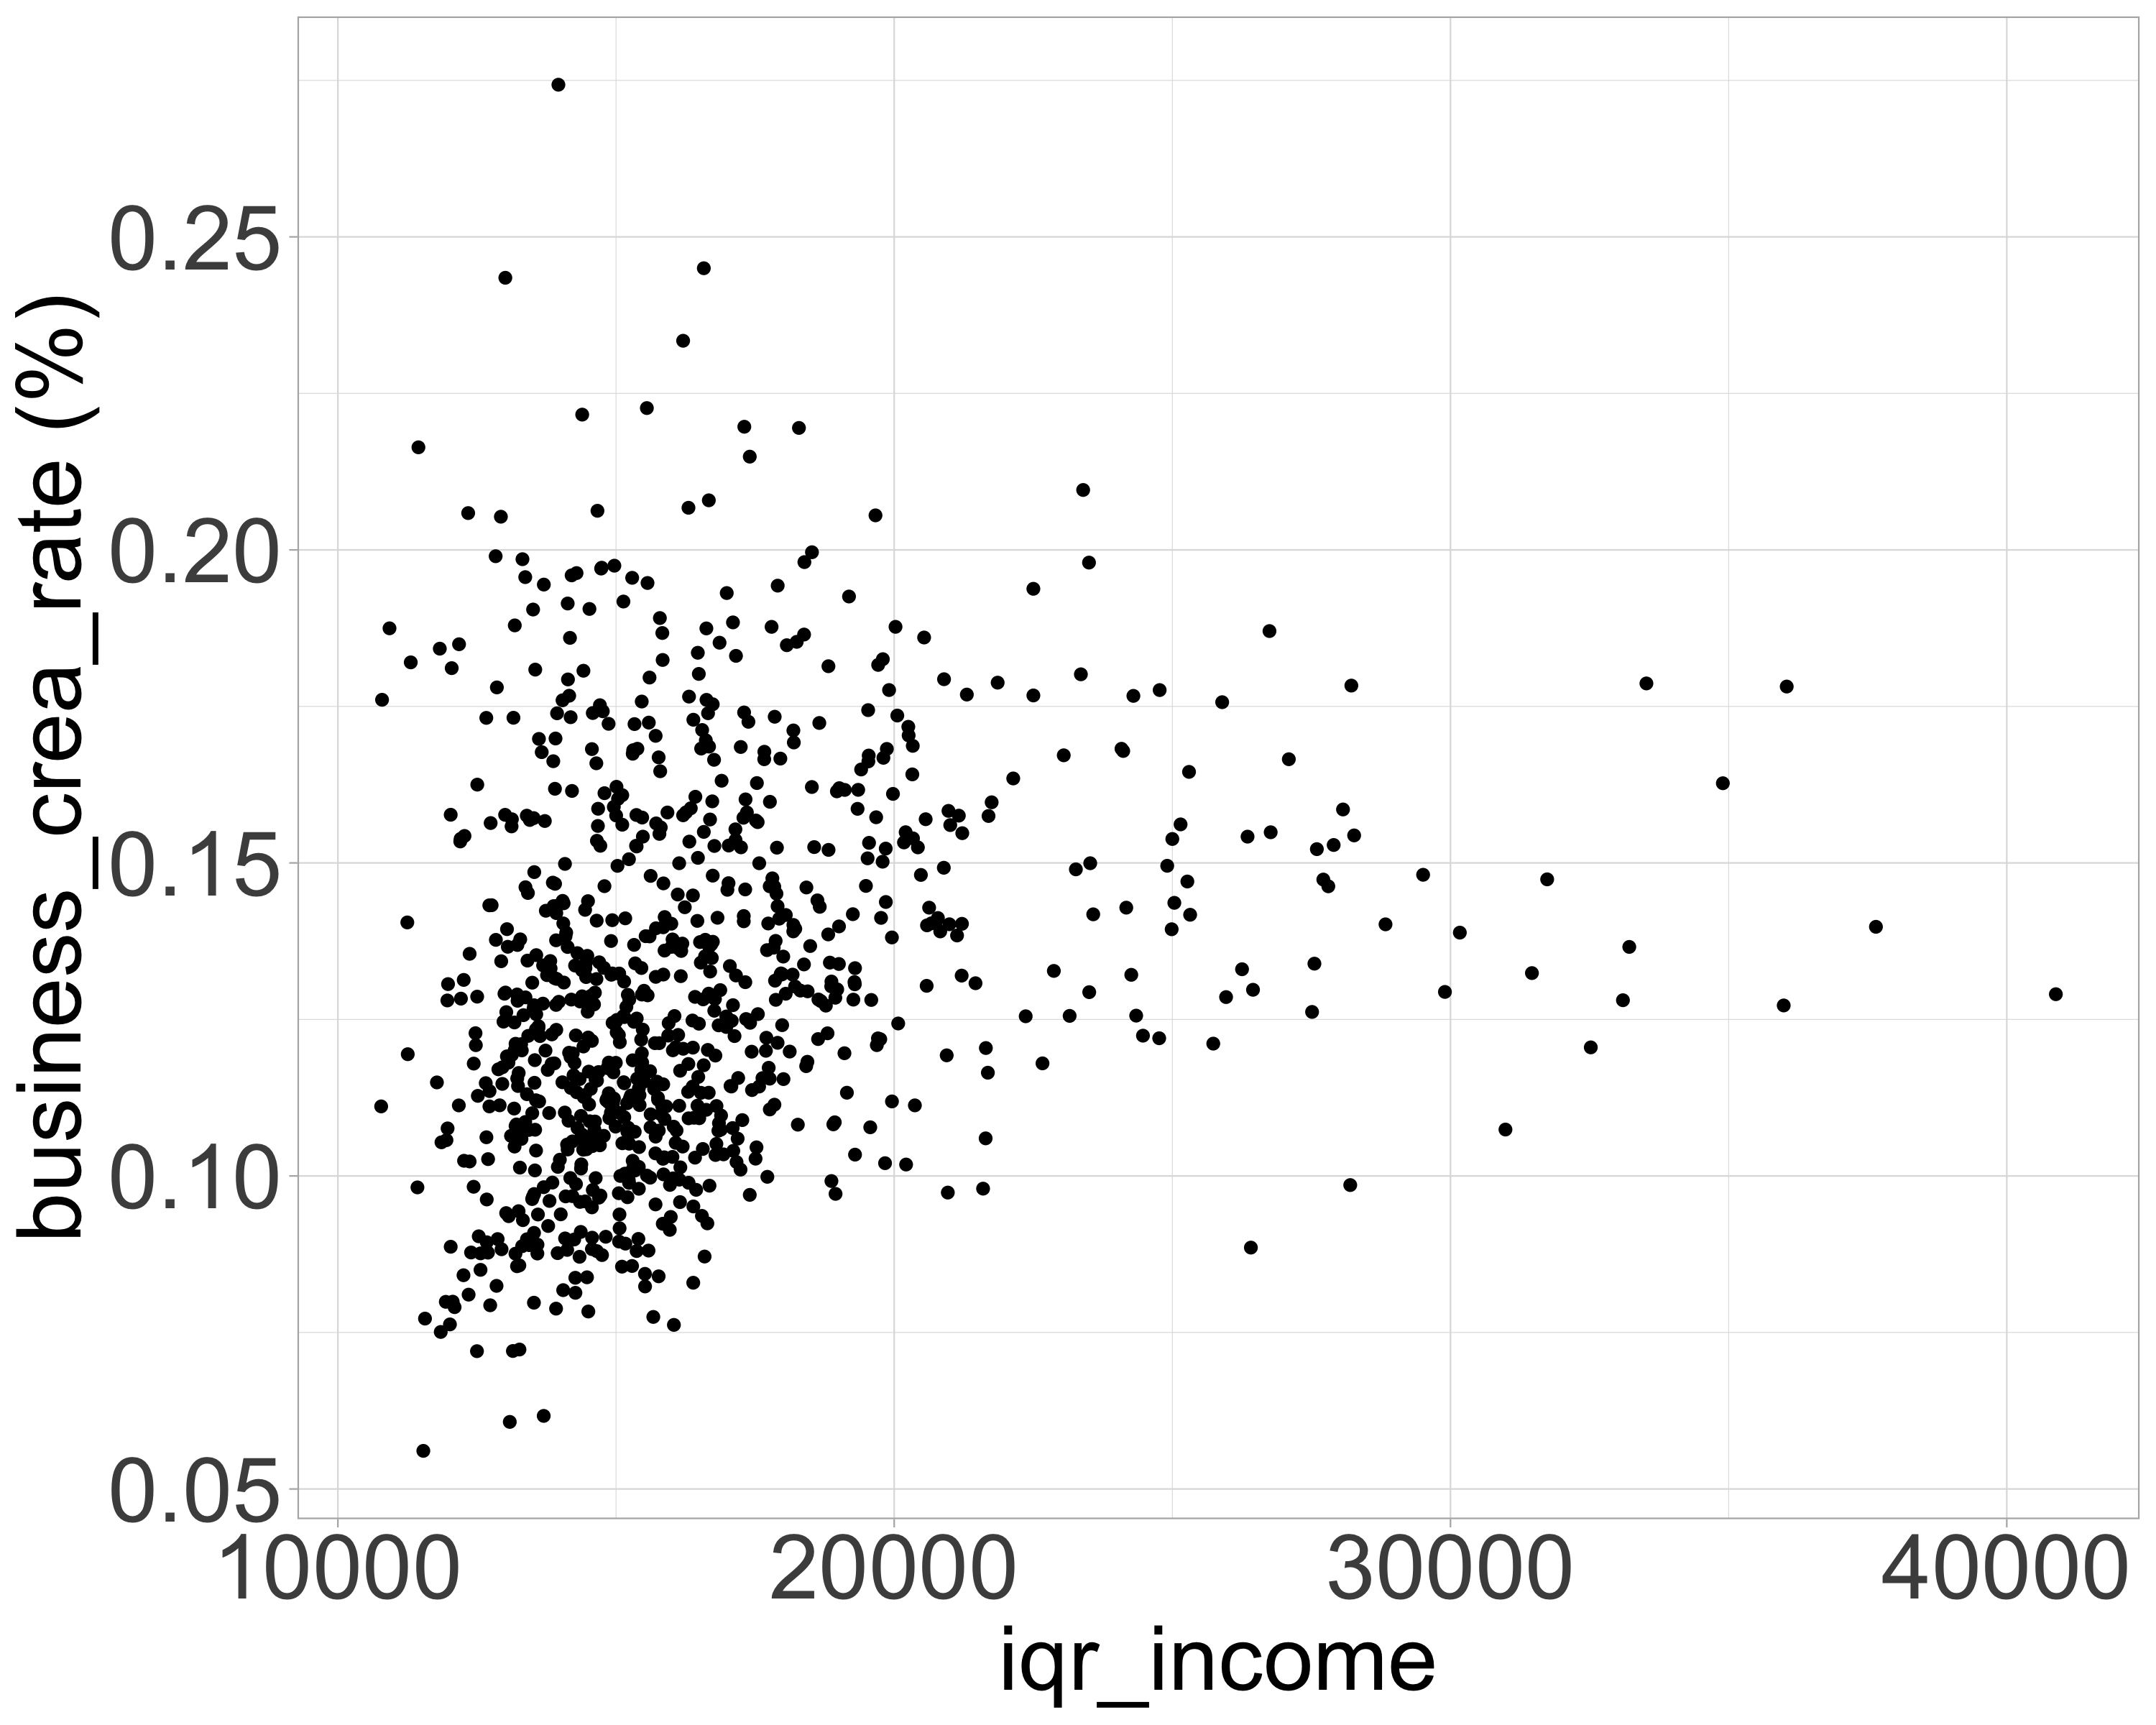
\includegraphics[width=\textwidth]{Exercise_3/OUTPUT/bcr_iqr.png}
    \end{minipage}
    \caption{Crime rate and business creation growth rate with respect to inequality indicator}
    \label{ineq}
  \end{figure}
\stepcounter{subsection}
\subsubsection{Discuss the validity of all potential instruments with respect to the relevance condition.}
For an instrumental variable to be relevant, they should have no direct impact on the dependant variable (orthogonality condition). Are there any reason to think that one of the three variables impact local crime rate ? It seems very unlikely for the motorway variable, unless a majority of crimes happen to occur during motoraces, which seems ridiculous. If we assume that the crime rate is driven by the living condition of a population, it seems unlikely that changing the political party of the mayor \textit{ceteris paribus} would have any impact on the crime rate. As for the tax rate variable, I would like to be more cautious. If, as I believe it is, the inequality level is part of the data generating process, then it could be that the local tax rate has an impact on the local level of (perceived) inequality and would impact the crime rate through this ommited variable. One should inspect the literature on the subject to build intuition about such a matter.
\subsubsection{Use the correlation between the business ce rate and the three variables to assess their potential strength as instruments. Does one seem better suited as an instrument than the other? Why?}

After computing the correlation between the instruments and the business creation growth rate, it appears that the motorway variable seems to be better suited than the other with correlation of 0.295 compared to 0.165 for the tax\_rate and -0.005 for the political party (see Figure \ref{cor}). The tax\_rate could still be used as an instrument with a correlation of 0.165 while the right variable would not add any information to the model.

\begin{figure}[htbp]
  \begin{minipage}{0.33\textwidth}%
    \centering
    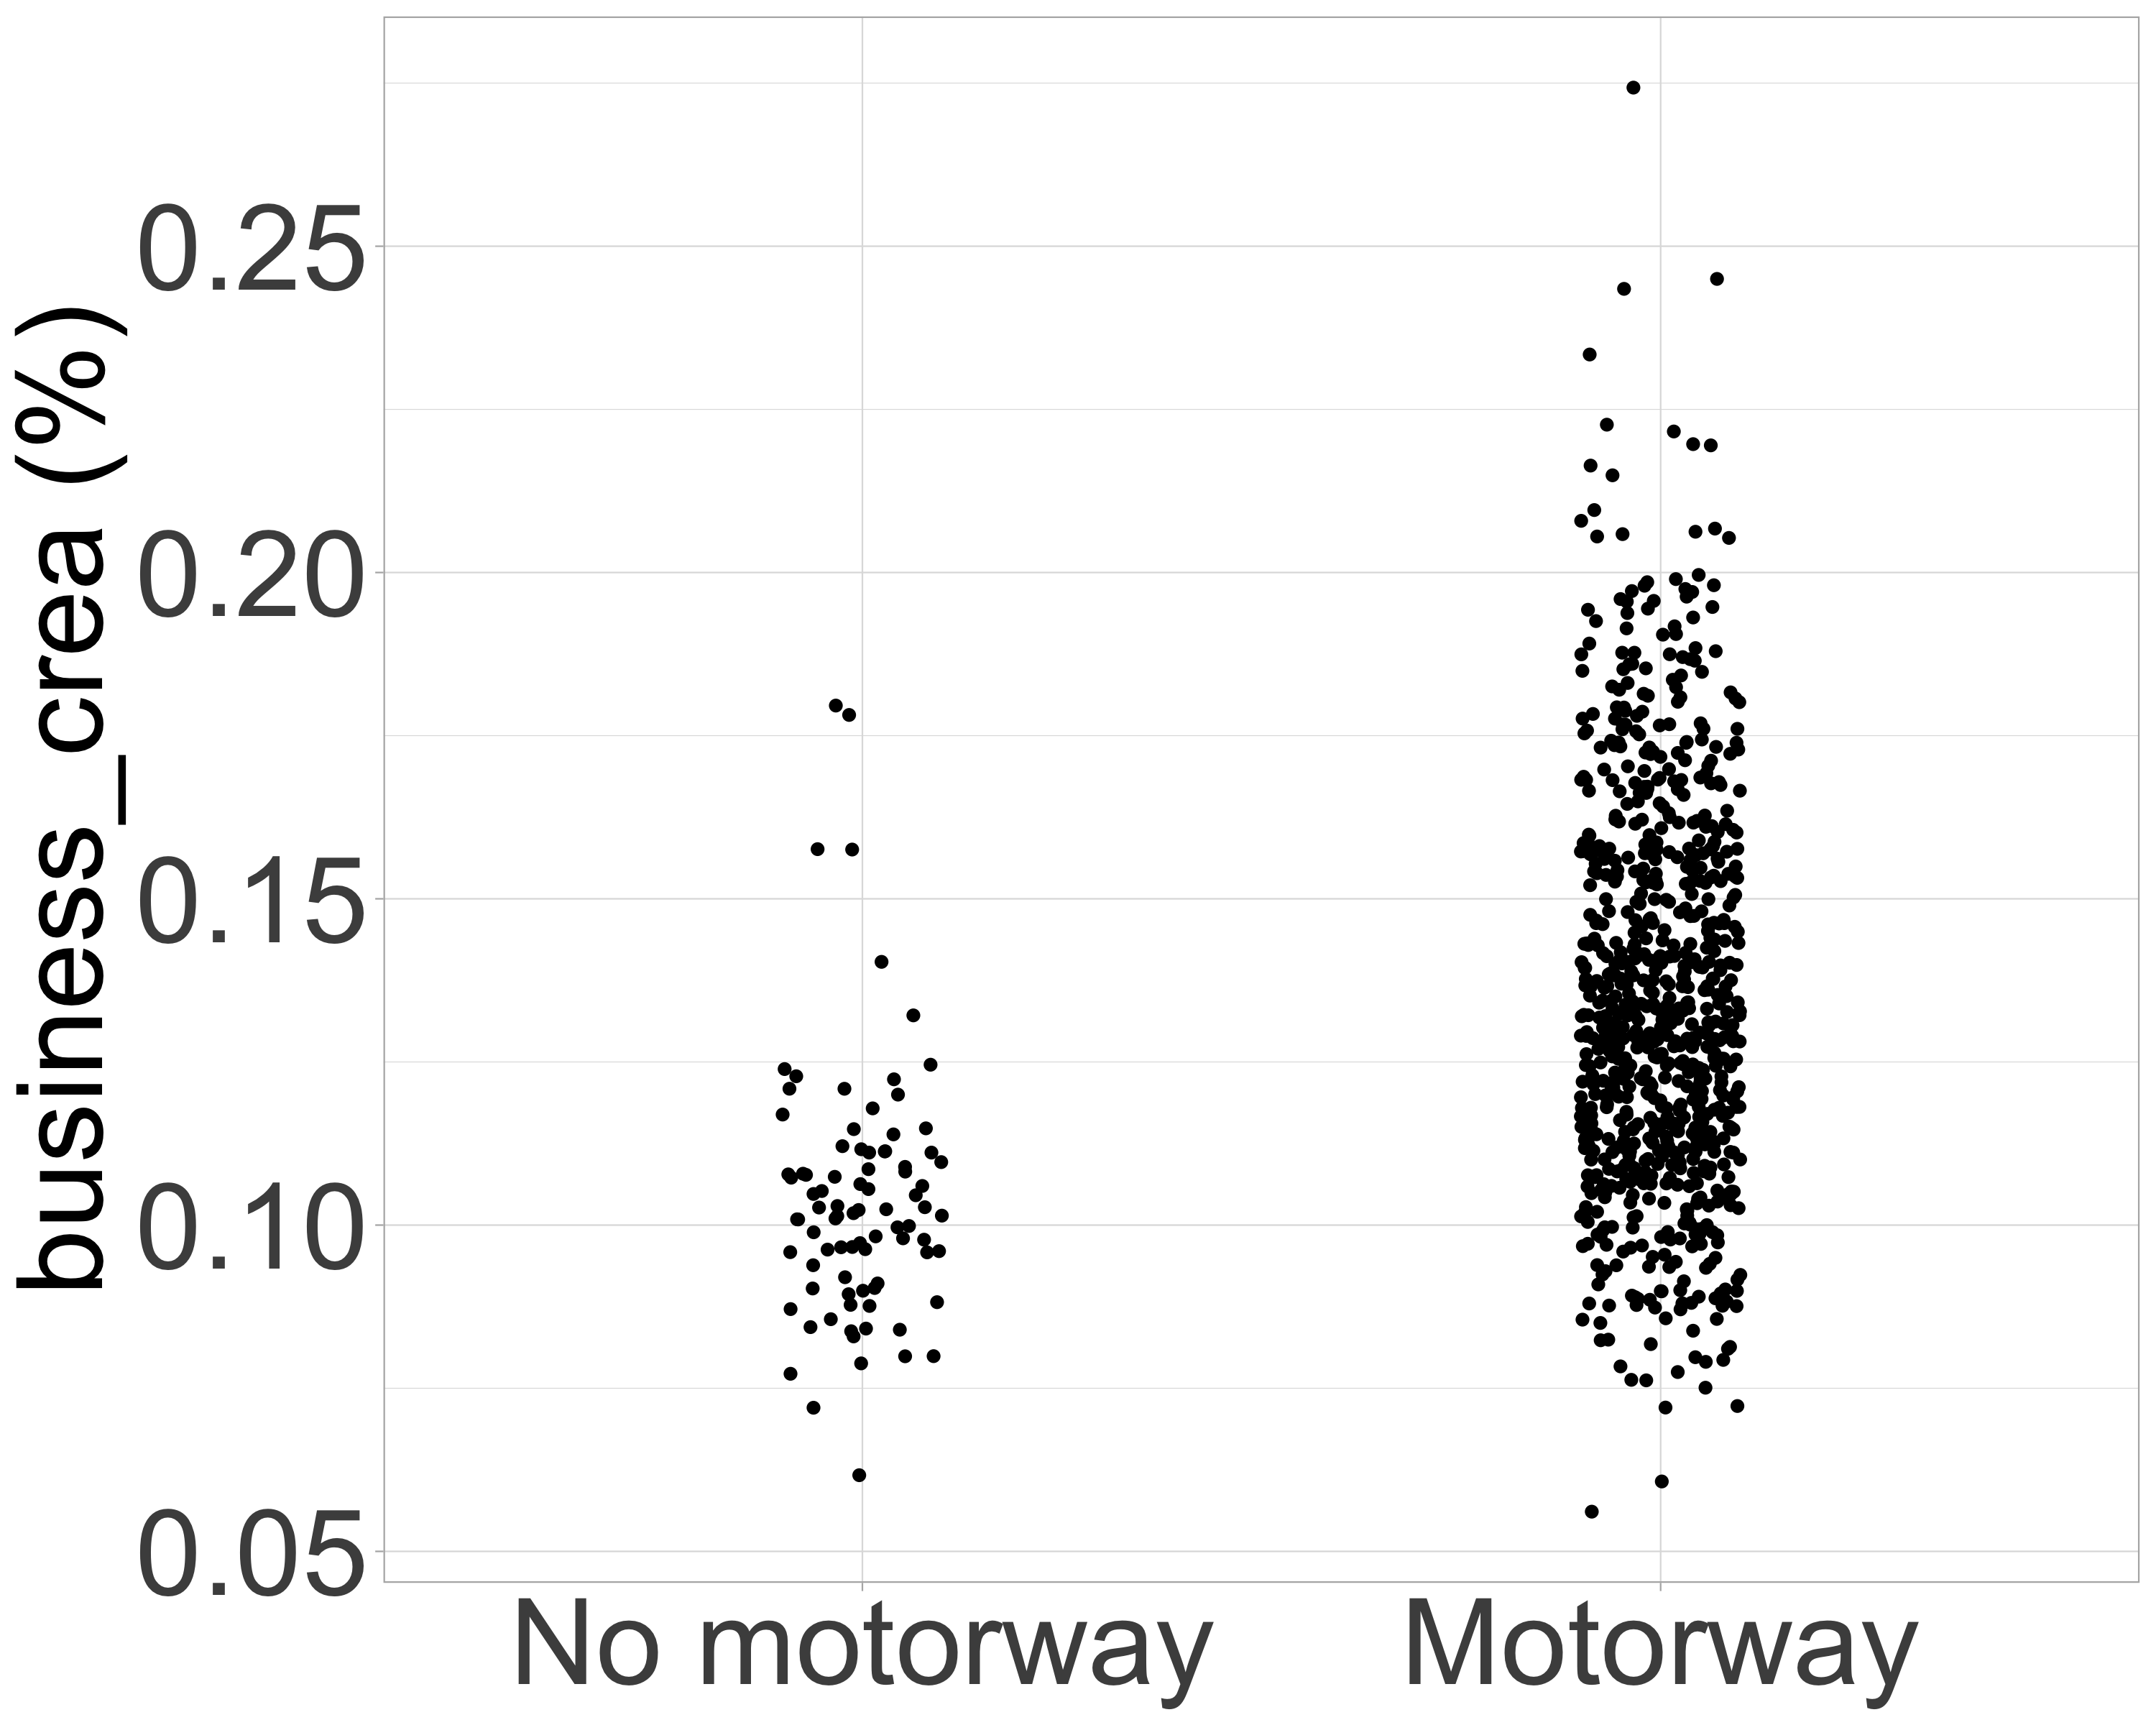
\includegraphics[width=\textwidth]{Exercise_3/OUTPUT/bcr_mtw.png}
  \end{minipage}%
  \begin{minipage}{0.33\textwidth}
    \centering
    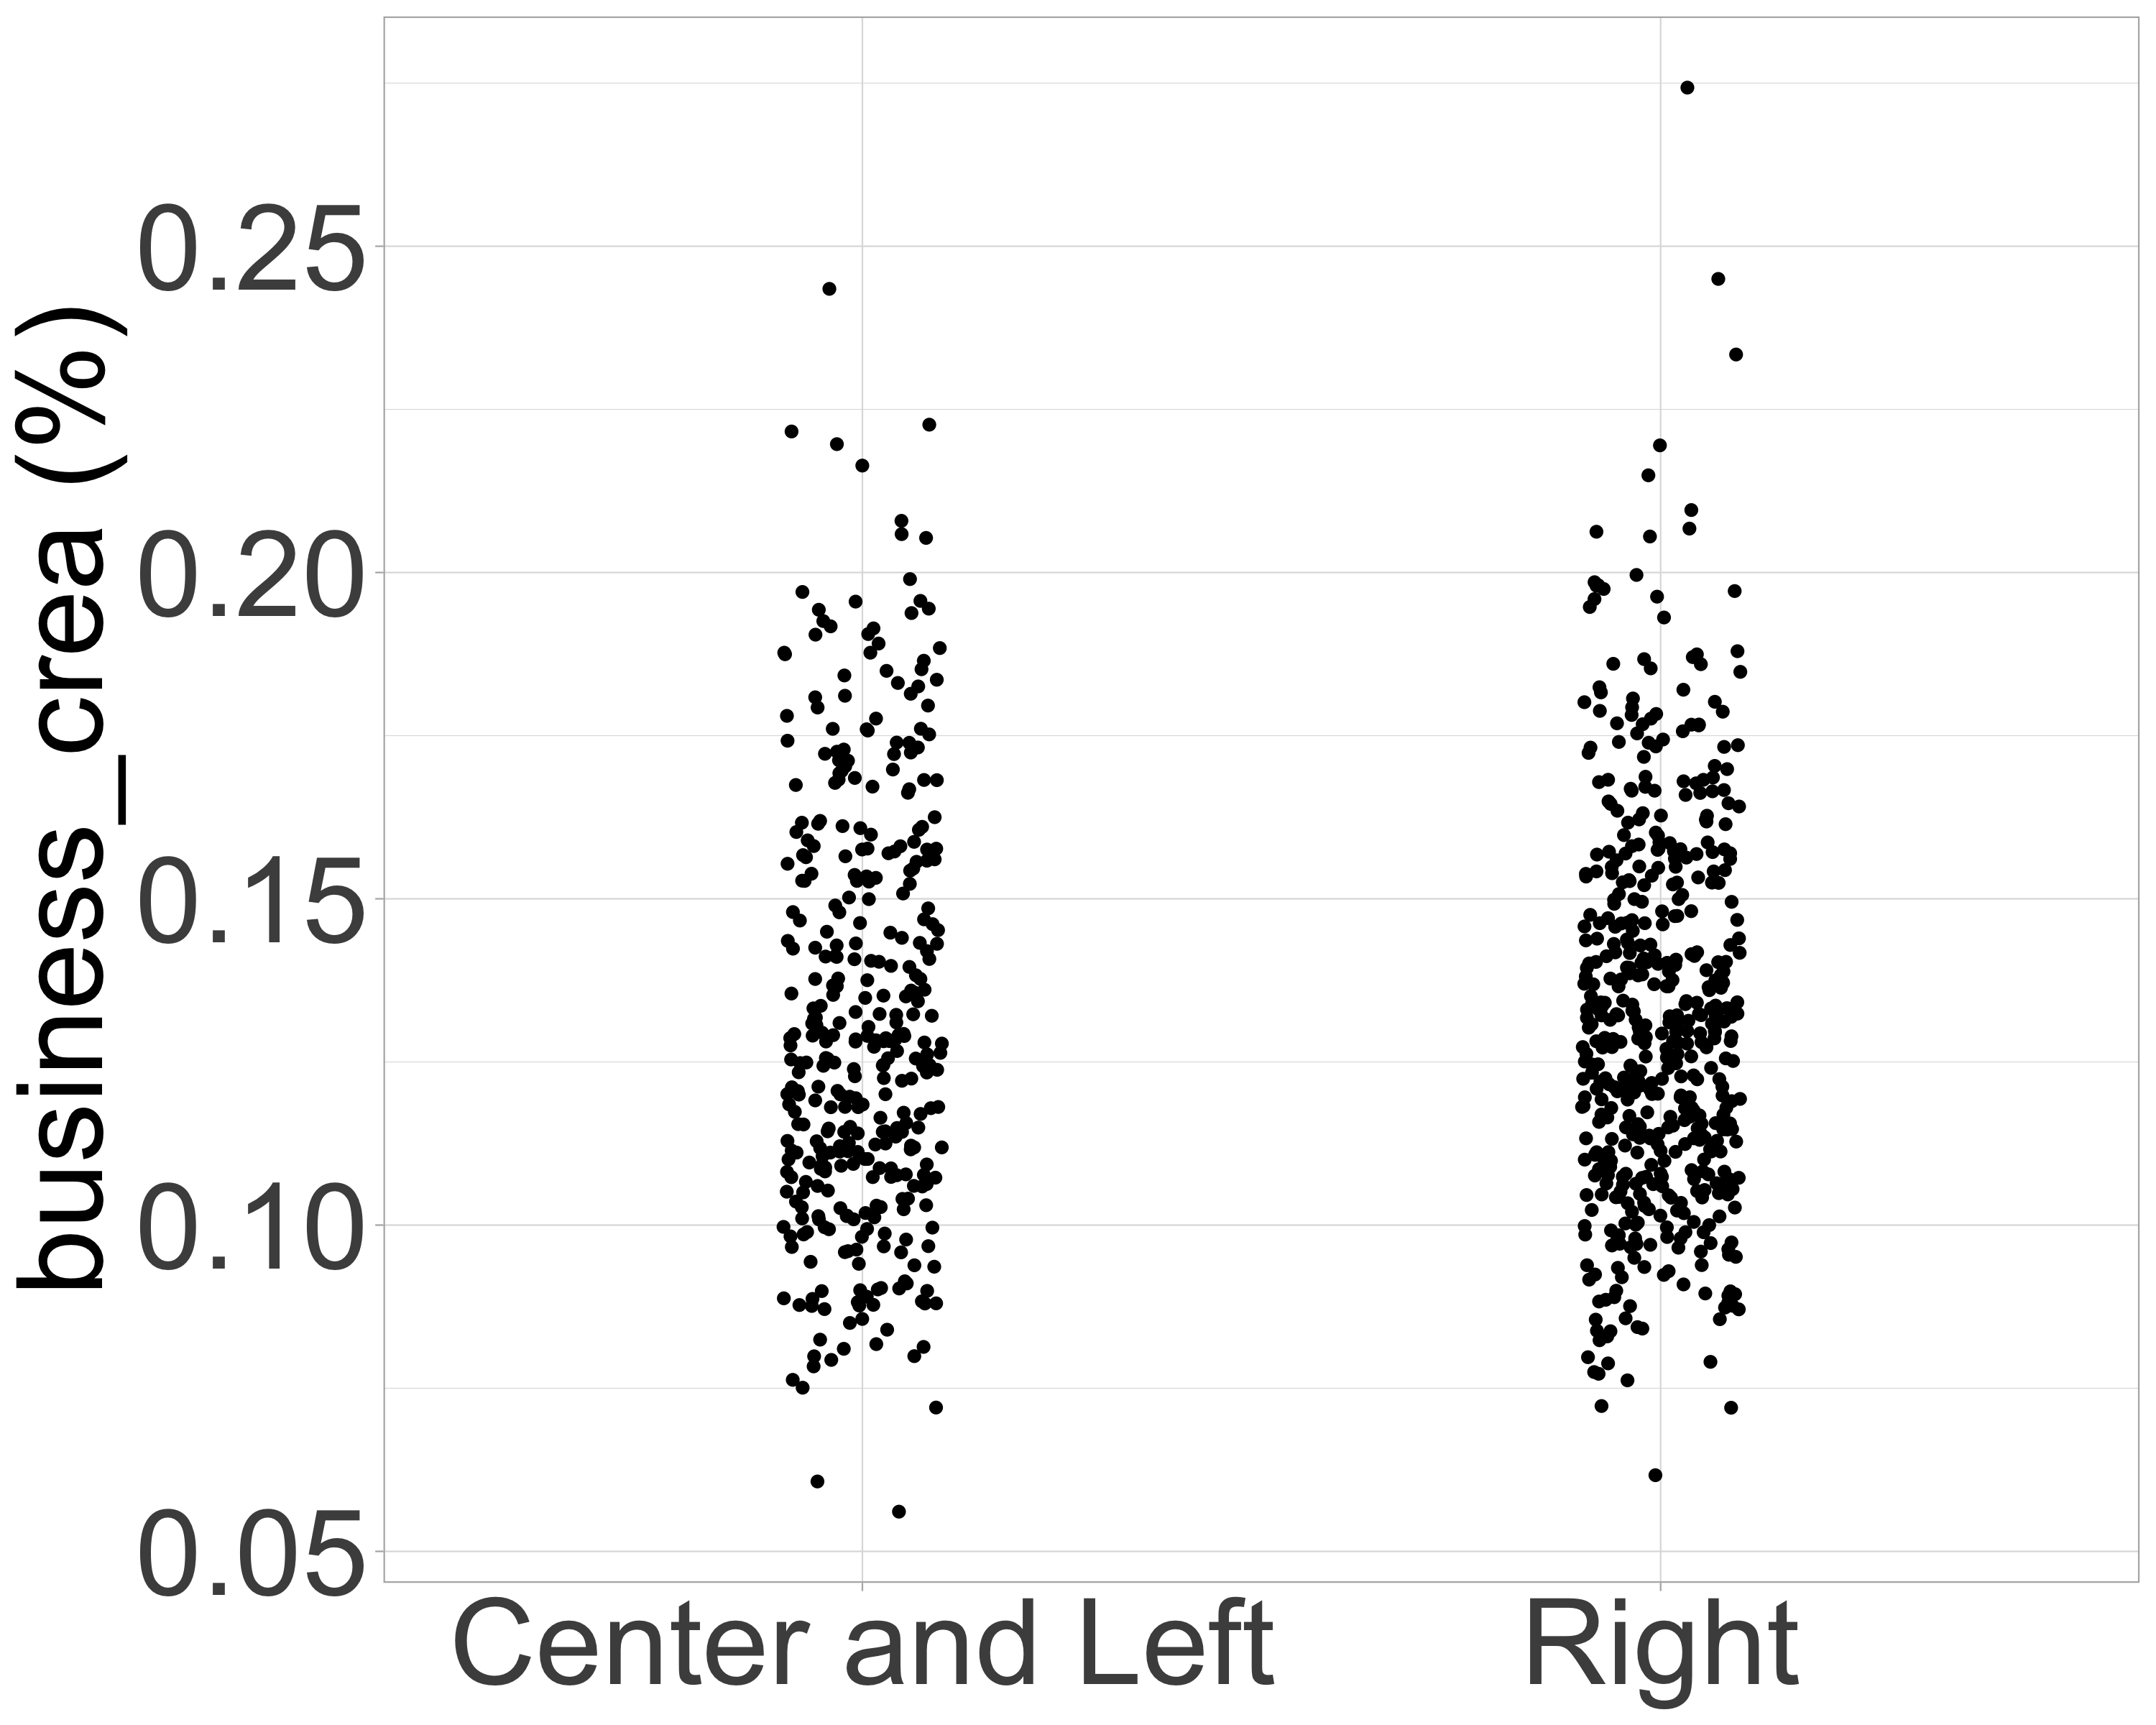
\includegraphics[width=\textwidth]{Exercise_3/OUTPUT/bcr_pty.png}
  \end{minipage}%
  \begin{minipage}{0.33\textwidth}
    \centering
    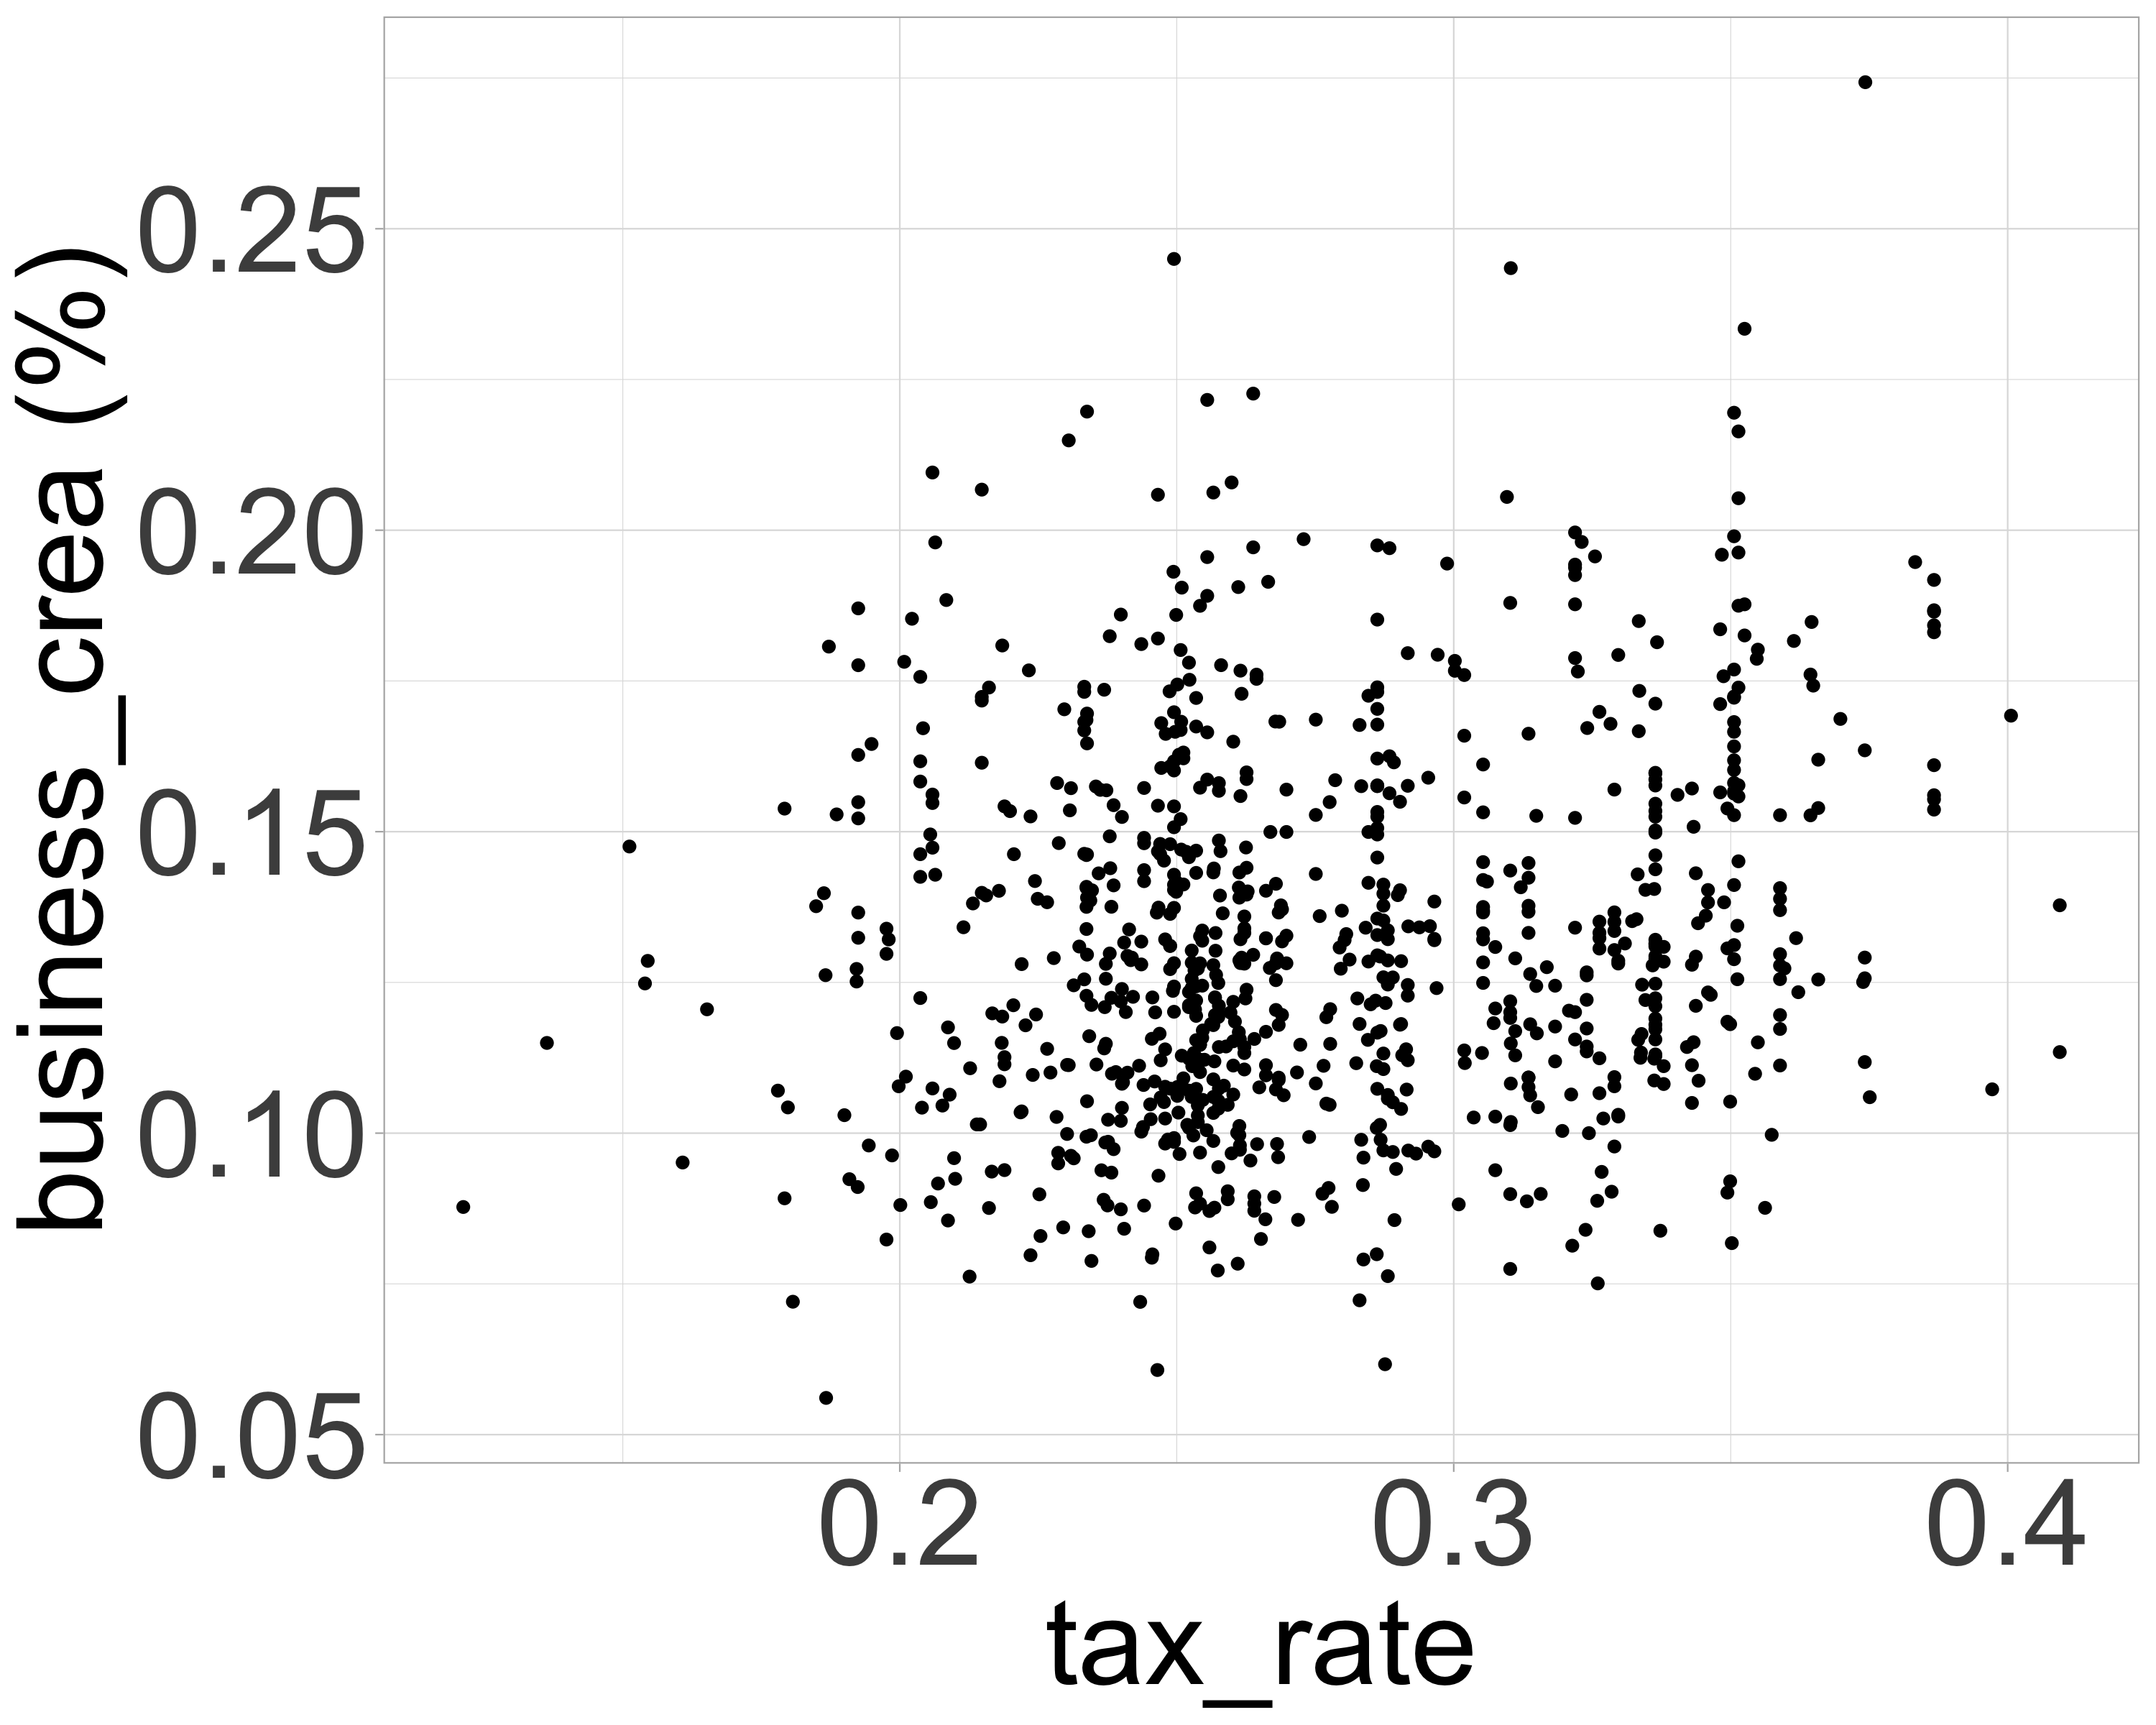
\includegraphics[width=\textwidth]{Exercise_3/OUTPUT/bcr_tx.png}
  \end{minipage}
  \caption{Business creation growth rate against instruments}
  \label{cor}
\end{figure}

\subsubsection{Thoroughly discuss the validity of the IV candidates regarding the exclusion restriction.}
We have discussed the exogeneity condition in the question 3.4.a which can be summarized as such :
there are no reasons to think the the party and motorway variables are part of the unexplained variations of the dependent variable while the tax rate variable could impact the level of inequality and thus impact the crime rate.
We cannot check the orthogonality condition as it relies on the distribution of the noise which we cannot access. 
To inspect the exclusion restriction, we can run a regression adding the instrumental variables to
the equation of interest and check that the coefficients are not significantly different from zero (see Table \ref{results3}).
It appears that the only instrumental variable that does not explain any variation in the
dependant variable is the party variable. It is not very convenient as
the party variable is also the weakest instrumental variable according to 3.4.b.
Although I have no explanation for the impact of the motorway variable, the coefficient
before the tax\_rate does not seem to confirm our analysis about the impact of this variable through the level
of inequality as it is positive. Maybe the tax\_rate is perceived as
unfair and actually increases the tension between the State and the population.

% Table created by stargazer v.5.2.3 by Marek Hlavac, Social Policy Institute. E-mail: marek.hlavac at gmail.com
% Date and time: Ven, jan 19, 2024 - 13:08:07
% Requires LaTeX packages: dcolumn 
\begin{table}[!htbp] \centering 
  \caption{Extended model - Exercise 3} 
  \label{results3} 
\small 
\begin{tabular}{@{\extracolsep{5pt}}lD{.}{.}{-3} } 
\\[-1.8ex]\hline 
\hline \\[-1.8ex] 
 & \multicolumn{1}{c}{\textit{Dependent variable:}} \\ 
\cline{2-2} 
\\[-1.8ex] & \multicolumn{1}{c}{crime\_rate} \\ 
\hline \\[-1.8ex] 
 business\_crea & 0.012^{***} \\ 
  & (0.005) \\ 
  & \\ 
 log(pop) & 0.0003^{*} \\ 
  & (0.0002) \\ 
  & \\ 
 income & 0.0004^{***} \\ 
  & (0.0001) \\ 
  & \\ 
 com\_typeC & -0.002^{***} \\ 
  & (0.0003) \\ 
  & \\ 
 com\_typeI & -0.001^{**} \\ 
  & (0.001) \\ 
  & \\ 
 motorway & 0.001^{***} \\ 
  & (0.0004) \\ 
  & \\ 
 partyRight & -0.001 \\ 
  & (0.001) \\ 
  & \\ 
 tax\_rate & 0.029^{***} \\ 
  & (0.003) \\ 
  & \\ 
 Constant & -0.006^{***} \\ 
  & (0.002) \\ 
  & \\ 
\hline \\[-1.8ex] 
Observations & \multicolumn{1}{c}{899} \\ 
R$^{2}$ & \multicolumn{1}{c}{0.261} \\ 
Adjusted R$^{2}$ & \multicolumn{1}{c}{0.254} \\ 
Residual Std. Error & \multicolumn{1}{c}{0.004 (df = 889)} \\
\hline 
\hline \\[-1.8ex] 
\textit{Note:}  & \multicolumn{1}{r}{$^{*}$p$<$0.1; $^{**}$p$<$0.05; $^{***}$p$<$0.01} \\ 
\end{tabular} 
\end{table} 


\stepcounter{subsection}

\subsubsection{Run 3 first-stage regressions, each using one of the above instruments separately. Report
the 3 sets of results in the same table. Which instrument seems to be the strongest?}
The results are displayed in Table \ref{first_stages} and correspond to what we displayed in Figure \ref{cor}.
The motorway variable seems to be the strongest instrument with a coefficient significantly different from zero at the 1\% level whereas the tax\_rate is only significant at the 5\% level and the party variable is not significant whatsoever. 

% Table created by stargazer v.5.2.3 by Marek Hlavac, Social Policy Institute. E-mail: marek.hlavac at gmail.com
% Date and time: Ven, jan 19, 2024 - 13:43:49
% Requires LaTeX packages: dcolumn 
\begin{table}[!htbp] \centering 
  \caption{First Stages - Exercise 3} 
  \label{first_stages} 
\footnotesize 
\begin{tabular}{@{\extracolsep{5pt}}lD{.}{.}{-3} D{.}{.}{-3} D{.}{.}{-3} } 
\\[-1.8ex]\hline 
\hline \\[-1.8ex] 
 & \multicolumn{3}{c}{\textit{Dependent variable:}} \\ 
\cline{2-4} 
\\[-1.8ex] & \multicolumn{3}{c}{business\_crea} \\ 
\\[-1.8ex] & \multicolumn{1}{c}{motorway} & \multicolumn{1}{c}{party} & \multicolumn{1}{c}{tax\_rate}\\ 
\hline \\[-1.8ex] 
 log(pop) & 0.011^{***} & 0.011^{***} & 0.011^{***} \\ 
  & (0.001) & (0.001) & (0.001) \\ 
  & & & \\ 
 income & -0.001 & -0.001 & -0.0001 \\ 
  & (0.001) & (0.001) & (0.001) \\ 
  & & & \\ 
 com\_typeC & -0.032^{***} & -0.034^{***} & -0.033^{***} \\ 
  & (0.002) & (0.002) & (0.002) \\ 
  & & & \\ 
 com\_typeI & -0.030^{***} & -0.033^{***} & -0.032^{***} \\ 
  & (0.004) & (0.004) & (0.004) \\ 
  & & & \\ 
 motorway & 0.014^{***} &  &  \\ 
  & (0.003) &  &  \\ 
  & & & \\ 
 partyLeft &  & -0.0003 &  \\ 
  &  & (0.004) &  \\ 
  & & & \\ 
 partyRight &  & 0.001 &  \\ 
  &  & (0.004) &  \\ 
  & & & \\ 
 tax\_rate &  &  & 0.039^{**} \\ 
  &  &  & (0.019) \\ 
  & & & \\ 
 Constant & 0.026^{**} & 0.034^{***} & 0.024^{*} \\ 
  & (0.012) & (0.013) & (0.013) \\ 
  & & & \\ 
\hline \\[-1.8ex] 
Observations & \multicolumn{1}{c}{899} & \multicolumn{1}{c}{899} & \multicolumn{1}{c}{899} \\ 
R$^{2}$ & \multicolumn{1}{c}{0.338} & \multicolumn{1}{c}{0.322} & \multicolumn{1}{c}{0.325} \\ 
Adjusted R$^{2}$ & \multicolumn{1}{c}{0.334} & \multicolumn{1}{c}{0.317} & \multicolumn{1}{c}{0.321} \\ 
Residual Std. Error & \multicolumn{1}{c}{0.025 (df = 893)} & \multicolumn{1}{c}{0.025 (df = 892)} & \multicolumn{1}{c}{0.025 (df = 893)} \\
\hline 
\hline \\[-1.8ex] 
\textit{Note:}  & \multicolumn{3}{r}{$^{*}$p$<$0.1; $^{**}$p$<$0.05; $^{***}$p$<$0.01} \\ 
\end{tabular} 
\end{table} 

\subsubsection{Extract the fitted values of any one of these first-stage regressions and use them to run
a second-stage regression. Assuming that the instrument is exogenous, are your results
reliable? Why?}
The results are displayed in Table \ref{2sls} along with the ivreg 2SLS regression. Although the coefficient of interest is significant at the 1\%, we have seen in Table \ref{results3} that the motorway variable
was part of the data generating process, thus even assuming the exogeneity condition is not enough to rely on those results.
\subsubsection{For the instrument chosen in part (b), instead of manually running the 2 stages, implement
the IV estimator using the ivreg package. Is your answer the same or different to the
answer in part (b) and why?}
The coefficients and variances are the almost identical as in the previous question because the computation follows the same process (see Table \ref{2sls}). That aside, the $R^2$ coefficient is negative which is a sign that the model is either wrong or overfitted. 

% Table created by stargazer v.5.2.3 by Marek Hlavac, Social Policy Institute. E-mail: marek.hlavac at gmail.com
% Date and time: Ven, jan 19, 2024 - 14:33:59
% Requires LaTeX packages: dcolumn 
\begin{table}[!htbp] \centering 
  \caption{2SLS Regression with and without ivreg Package} 
  \label{2sls} 
\small 
\begin{tabular}{@{\extracolsep{5pt}}lD{.}{.}{-3} D{.}{.}{-3} } 
\\[-1.8ex]\hline 
\hline \\[-1.8ex] 
 & \multicolumn{2}{c}{\textit{Dependent variable:}} \\ 
\cline{2-3} 
\\[-1.8ex] & \multicolumn{2}{c}{crime\_rate} \\ 
\\[-1.8ex] & \multicolumn{1}{c}{\textit{manual 2SLS}} & \multicolumn{1}{c}{\textit{ivreg 2SLS}} \\ 
\\[-1.8ex] & \multicolumn{1}{c}{(1)} & \multicolumn{1}{c}{(2)}\\ 
\hline \\[-1.8ex] 
 fitted\_business\_crea & 0.111^{***} &  \\ 
  & (0.033) &  \\ 
  & & \\ 
 business\_crea &  & 0.111^{***} \\ 
  &  & (0.039) \\ 
  & & \\ 
 log(pop) & -0.001 & -0.001 \\ 
  & (0.0004) & (0.0005) \\ 
  & & \\ 
 income & 0.0001 & 0.0001 \\ 
  & (0.0001) & (0.0001) \\ 
  & & \\ 
 com\_typeC & 0.001 & 0.001 \\ 
  & (0.001) & (0.001) \\ 
  & & \\ 
 com\_typeI & 0.001 & 0.001 \\ 
  & (0.001) & (0.001) \\ 
  & & \\ 
 Constant & -0.002 & -0.002 \\ 
  & (0.002) & (0.003) \\ 
  & & \\ 
\hline \\[-1.8ex] 
Observations & \multicolumn{1}{c}{899} & \multicolumn{1}{c}{899} \\ 
R$^{2}$ & \multicolumn{1}{c}{0.149} & \multicolumn{1}{c}{-0.174} \\ 
Adjusted R$^{2}$ & \multicolumn{1}{c}{0.144} & \multicolumn{1}{c}{-0.181} \\ 
Residual Std. Error (df = 893) & \multicolumn{1}{c}{0.004} & \multicolumn{1}{c}{0.005} \\ 
F Statistic & \multicolumn{1}{c}{31.260$^{***}$ (df = 5; 893)} &  \\ 
\hline 
\hline \\[-1.8ex] 
\textit{Note:}  & \multicolumn{2}{r}{$^{*}$p$<$0.1; $^{**}$p$<$0.05; $^{***}$p$<$0.01} \\ 
\end{tabular} 
\end{table} 

\subsubsection{Use all instruments you think are valid to implement the IV estimator using the ivreg
package and report your results. How different are the results from part (c)?}
The two estimators that are correlated enough with the endogenous variable are the motorway and tax\_rate variables
(see Table \ref{first_stages}), assuming the orthogonality condition for both of them, they are the only estimators to use in a 2SLS regression.
The results are displayed in Table \ref{2sls_mtw_tr} and we get an even higher coefficient for the growth rate of the economy which would mean that, the better the shape of the economy in an area, the higher the crime rate even after recovering exogeneity using insrumental variables. 

% Table created by stargazer v.5.2.3 by Marek Hlavac, Social Policy Institute. E-mail: marek.hlavac at gmail.com
% Date and time: Ven, jan 19, 2024 - 15:55:24
% Requires LaTeX packages: dcolumn 
\begin{table}[!htbp] \centering 
  \caption{2SLS Regression With motorway and tax rate as Instruments} 
  \label{2sls_mtw_tr} 
\small 
\begin{tabular}{@{\extracolsep{5pt}}lD{.}{.}{-3} } 
\\[-1.8ex]\hline 
\hline \\[-1.8ex] 
 & \multicolumn{1}{c}{\textit{Dependent variable:}} \\ 
\cline{2-2} 
\\[-1.8ex] & \multicolumn{1}{c}{crime\_rate} \\ 
\hline \\[-1.8ex] 
 business\_crea & 0.217^{***} \\ 
  & (0.051) \\ 
  & \\ 
 log(pop) & -0.002^{***} \\ 
  & (0.001) \\ 
  & \\ 
 income & 0.0001 \\ 
  & (0.0002) \\ 
  & \\ 
 com\_typeC & 0.004^{**} \\ 
  & (0.002) \\ 
  & \\ 
 com\_typeI & 0.004^{**} \\ 
  & (0.002) \\ 
  & \\ 
 Constant & -0.005 \\ 
  & (0.004) \\ 
  & \\ 
\hline \\[-1.8ex] 
Observations & \multicolumn{1}{c}{899} \\ 
R$^{2}$ & \multicolumn{1}{c}{-1.344} \\ 
Adjusted R$^{2}$ & \multicolumn{1}{c}{-1.357} \\ 
Residual Std. Error & \multicolumn{1}{c}{0.006 (df = 893)} \\ 
\hline 
\hline \\[-1.8ex] 
\textit{Note:}  & \multicolumn{1}{r}{$^{*}$p$<$0.1; $^{**}$p$<$0.05; $^{***}$p$<$0.01} \\ 
\end{tabular} 
\end{table} 
